
\section{База данни -  таблици и модели}
Базата данни бива достъпвана от приложението чрез
специални класове, т.н. модели. Те представят
различните типове данни в контекста на
приложението, както и отношенията между тях. Често
съдържат методи, специализирани в работа с конкретния
тип данни.
Моделите наследяват от базов клас Core::Entity.
Различните колони в MySQL таблиците се описват като
полета в класа, а имената на таблиците, първичните
ключове и отношенията между тях се описват чрез атрибути.
Допълнителна функционалност и логика към моделите се
добавя чрез методи в самия модел.

Стуктурата на базата данни можете да видите на
следващата страница. След нея има по - обстойно
описание на отделните модели и съответните таблици.

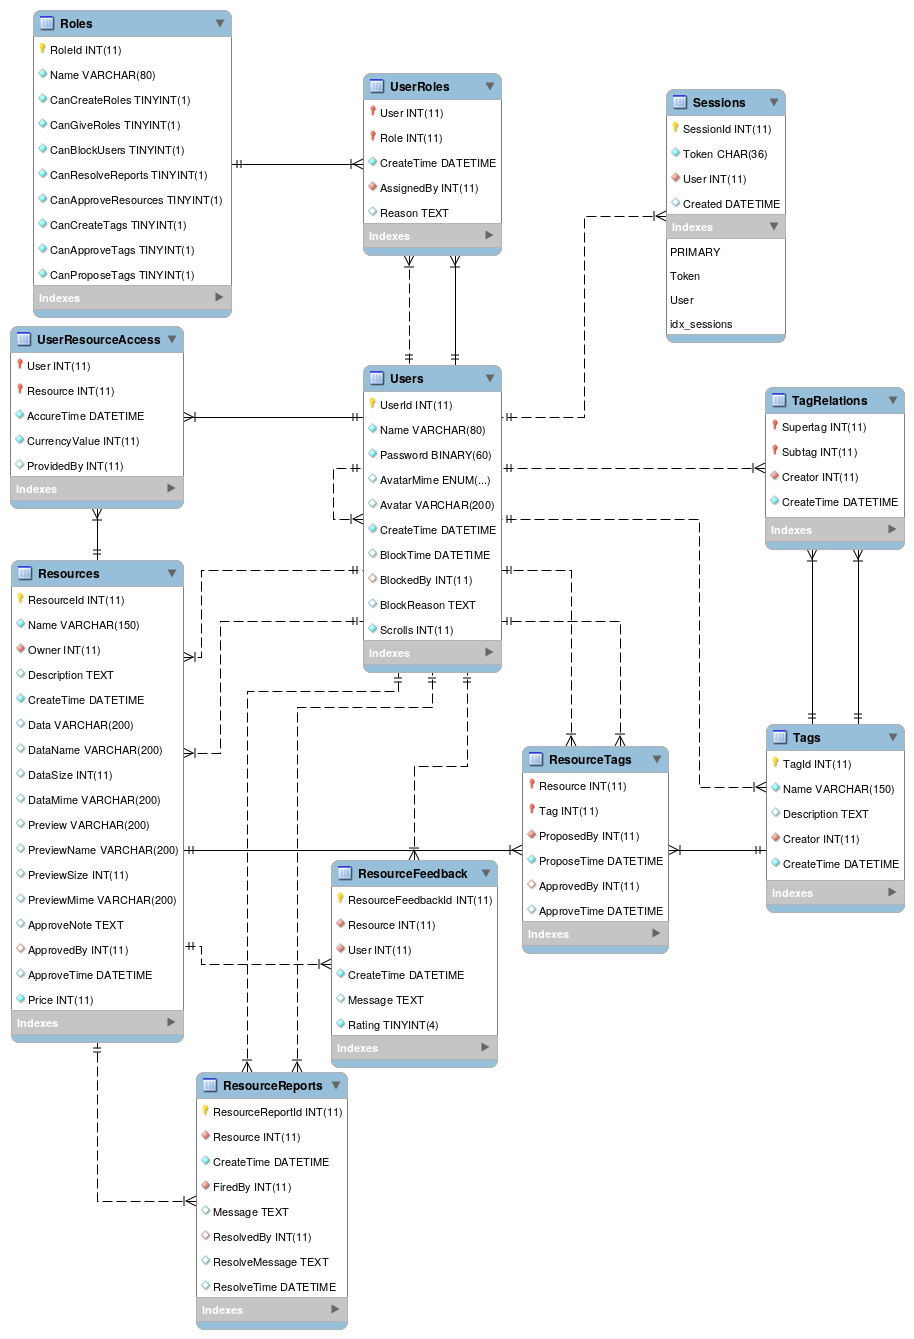
\includepdf{../../db.png}


\subsection{Потребител}
Представен от класа Model/User.php

Съдържа информация свързана с потребителския профил,
като потребителско име, хеширана парола, налична валута, 
потребителски аватар, време и причина за блокиране
на профила, ако е налично.

Създава се в базата данни чрез заявката:
\inputSQL{Users.sql}


\subsection{Сесия}
Представена от класа Model/Session.php

Съхранява и обработва информация за настоящата сесия,
като използва бисквитка или полето token при REST заявки,
за да позволи наличието на потребителски профили.

Създава се в базата данни чрез заявката:
\inputSQL{Sessions.sql}


\subsection{Потребителска роля}
Представена от класа Model/Role.php

Съдържа информация за достъпните действия на всички
потребители, които имат тази роля.
При потребители с повече от една роля действието е
достъпно ако една или повече от ролите го позволяват.

Създава се в базата данни чрез заявката:
\inputSQL{Roles.sql}


\subsection{Ресурс}
Представен от класа Model/Resource.php

Съдържа информация за конкретна учебна тема или учебен
ресурс. Такава информация е името, автора, дата на
създаване, описание, цена, одобрение от модератор, както
и тип, размер, път и име на пълната и
демонстративната версия на ресурса.

Създава се в базата данни чрез заявката:
\inputSQL{Resources.sql}


\subsection{Ключова дума}
Представена от класа Model/Tag.php

Обозначава ключова дума, както и описанието към нея,
ако има такова. Използват се при филтриране на ресурси.

Създава се в базата данни чрез заявката:
\inputSQL{Tags.sql}


\subsection{Оценка на ресурс}
Представена от класа Model/ResourceFeedback.php

Съдържа мнение за съдържанието на ресурса под формата
на кратко съобщение и оценка, както и дата на добавяне.

Създава се в базата данни чрез заявката:
\inputSQL{ResourceFeedback.sql}


\subsection{Съобщение за нередност}
Представено от класа Model/Tag.php

Съдържа време, ресурс, потребител и причина за подаване,
както и време, бележка и модератор, който го е разгледал.

Създава се в базата данни чрез заявката:
\inputSQL{ResourceReports.sql}


\subsection{Свързващи модели}
Представени от класовете в Model/Junction

Представят връзките от тип много към много между
моделите в приложението, както и необходима допълнителна
информация относно отношението между два обекта.
Такива отношения са
\begin{itemize}
    \item Потребител - Роля
    \item Ключова дума - Ресурс
    \item Потребител - Закупени ресурси
    \item Основни ключови думи - Специфични ключови думи
\end{itemize}

Те могат да бъдат създадени чрез заявките:
\inputSQL{UserRoles.sql}
\inputSQL{ResourceTags.sql}
\inputSQL{UserResourceAccess.sql}
\inputSQL{TagRelations.sql}
